\documentclass{article}
\usepackage[utf8]{inputenc}
\usepackage{enumerate}
\usepackage{amsmath}
\usepackage{mathtools} 
\usepackage{amssymb}
\usepackage{systeme}
\usepackage[english]{babel}
\usepackage{xparse}
\usepackage{xfrac}
\usepackage{setspace}
\usepackage{multicol}
\usepackage{array}
\usepackage{tabularx}
\usepackage{bigints}
\usepackage{fontspec}


\usepackage{geometry}
 \geometry
{
 	a4paper,
 	total={170mm,257mm},
 	left=20mm,
	right = 20mm,
 	top=20mm,
 }



\begin{document}
%\onehalfspacing

\setmainfont{Arian AMU}

\begin{titlepage}
	\begin{center}
	
		\begin{LARGE}
		       \textbf{Հայաստանի Ազգային Պոլիտեխնիկական Համալսարան}
		\end{LARGE}
		
		       \vspace{0.5cm}
		
		\begin{Large}
		        Կիրառական մաթեմատիկայի և ֆիզիկայի ֆակուլտետ
		\end{Large}		            
		
		       \vspace{0.8cm}
		     
		
\includegraphics[width=0.4\textwidth]{images/university}


		       \vspace{1.5cm}
		
		\begin{huge}
		       \textbf{Կուրսային  աշխատանք}
		\end{huge}


	
	\end{center}


	\vspace{4cm}

	\begin{flushleft}
	\begin{large}
		Առարկա՝    Թվային մեթոդներ\\
		Դասախոս՝  Բաբայան Արմենակ\\
		Ուսանող՝     Սևոյան Կամո\\
		Խումբ՝         ՄԹ 940-2\\
	\end{large}
	\end{flushleft}



	\vfill

	\begin{center}
		Երևան 2022
	\end{center}

\end{titlepage}

\begin{center}
\textbf{Տարբերակ 23}
\end{center}

\section*{Խնդիր 1}

Տրված $\left(x_{k}, y_{k}\right)$ ինտերպոլյացիոն տվյալներով։

\begin{enumerate}

\item	կառուցել Լագրանժի ինտերպոլյացիոն բազմանդամ
\item        կառուցել բաժանված տարբերությունների աղյուսակը
\item        կառուցել Նյուտոնի ինտերպոլյացիոն բազմանդամը
\item        համեմատել Լագրանժի և Նյուտոնի ինտերպոլյացիոն բազմանդամների արժեքները $\tilde{x}$ կետում։

\end{enumerate}

$$
\begin{array}{c|c|c|c|c|c|c|c|c}
		x_{k}	&	1.21		&	2.51		&	2.91		&	3.35		&	3.78		&	4.61		&	5.51		&	6.91  \\ \hline
 		y_{k}	&	1.12		&	1.39		&	1.04		&	1.21		&	1.58		&	1.82		&	2.25		&	2.78	 \\
\end{array},  \tilde{x} = 4.05
$$


\subsection*{Լուծում.}

\begin{enumerate}
\item

Համաձայն Լագրանժի ինտերպոլյացիոն բազմանդամի սահմանման․

\begin{equation*}
	L_{n-1}\left(x\right) = \sum_{k = 1}^{n} f\left(x_{k}\right)\prod_{\substack{j = 1 \\
																													 j\neq k}}^{n}\frac{x - x_{j}}{x_{k} - x_{j}}
\end{equation*}

	Տվյալ ինտերպոլյացիոն տվյալներին համապատասխան Լագրանժի բազմանդամը կլինի՝


$L_{7}\left(x\right)  = \\
1.12\dfrac{\left(x-2.51\right)\left(x-2.91\right)\left(x-3.35\right)\left(x-3.78\right)\left(x-4.61\right)\left(x-5.51\right)\left(x-6.91\right)}										{\left(1.21-2.51\right)\left(1.21-2.91\right)\left(1.21-3.35\right)\left(1.21-3.78\right)\left(1.21-4.61\right)\left(1.21-5.51\right)\left(1.21-6.91\right)} + \\ \\
1.39\dfrac{\left(x-1.21\right)\left(x-2.91\right)\left(x-3.35\right)\left(x-3.78\right)\left(x-4.61\right)\left(x-5.51\right)\left(x-6.91\right)}										{\left(2.51-1.21\right)\left(2.51-2.91\right)\left(2.51-3.35\right)\left(2.51-3.78\right)\left(2.51-4.61\right)\left(2.51-5.51\right)\left(2.51-6.91\right)} + \\ \\
1.04\dfrac{\left(x-1.21\right)\left(x-2.51\right)\left(x-3.35\right)\left(x-3.78\right)\left(x-4.61\right)\left(x-5.51\right)\left(x-6.91\right)}										{\left(2.91-1.21\right)\left(2.91-2.51\right)\left(2.91-3.35\right)\left(2.91-3.78\right)\left(2.91-4.61\right)\left(2.91-5.51\right)\left(2.91-6.91\right)} + \\ \\
1.21\dfrac{\left(x-1.21\right)\left(x-2.51\right)\left(x-2.91\right)\left(x-3.78\right)\left(x-4.61\right)\left(x-5.51\right)\left(x-6.91\right)}										{\left(3.35-1.21\right)\left(3.35-2.51\right)\left(3.35-2.91\right)\left(3.35-3.78\right)\left(3.35-4.61\right)\left(3.35-5.51\right)\left(3.35-6.91\right)} + \\ \\
1.58\dfrac{\left(x-1.21\right)\left(x-2.51\right)\left(x-2.91\right)\left(x-3.35\right)\left(x-4.61\right)\left(x-5.51\right)\left(x-6.91\right)}										{\left(3.78-1.21\right)\left(3.78-2.51\right)\left(3.78-2.91\right)\left(3.78-3.35\right)\left(3.78-4.61\right)\left(3.78-5.51\right)\left(3.78-6.91\right)} + \\ \\
1.82\dfrac{\left(x-1.21\right)\left(x-2.51\right)\left(x-2.91\right)\left(x-3.35\right)\left(x-3.78\right)\left(x-5.51\right)\left(x-6.91\right)}										{\left(4.61-1.21\right)\left(4.61-2.51\right)\left(4.61-2.91\right)\left(4.61-3.35\right)\left(4.61-3.78\right)\left(4.61-5.51\right)\left(4.61-6.91\right)} + \\ \\
2.25\dfrac{\left(x-1.21\right)\left(x-2.51\right)\left(x-2.91\right)\left(x-3.35\right)\left(x-3.78\right)\left(x-4.61\right)\left(x-6.91\right)}										{\left(5.51-1.21\right)\left(5.51-2.51\right)\left(5.51-2.91\right)\left(5.51-3.35\right)\left(5.51-3.78\right)\left(5.51-4.61\right)\left(5.51-6.91\right)} + \\ \\
2.78\dfrac{\left(x-1.21\right)\left(x-2.51\right)\left(x-2.91\right)\left(x-3.35\right)\left(x-3.78\right)\left(x-4.61\right)\left(x-5.51\right)}										{\left(6.91-1.21\right)\left(6.91-2.51\right)\left(6.91-2.91\right)\left(6.91-3.35\right)\left(6.91-3.78\right)\left(6.91-4.61\right)\left(6.91-5.51\right)} \\ \\$


\item


Համաձայն բաժանված տարբերության սահմանման․

		$$f\left(x_{k}, x_{k+1}\right) = \frac{f\left(x_{k+1}\right) - f\left(x_{k}\right)}{x_{k+1} - x_{k}}$$
	         $$f\left(x_{i}, x_{i+1}, \dots, x_{i+k}\right) = \frac{f\left(x_{i+1}, \dots, x_{i+k}\right) - f\left(x_{i}, \dots, x_{i+k-1}\right)}{x_{i+k} - x_{i}}$$



Հետևաբար աղյուսակը կլինի․


$$
\begin{array}{c|c|c|c|c|c|c|c|c}
		&	0		&	1		&	2		&	3		&	4		&	5		&	6		&	7		\\	\hline
	1.21	&	1.12		&			&			&			&			&			&			&			\\	\hline
		&			&	0.21		&			&			&			&			&			&			\\	\hline
	2.51	&	1.39		&			&	-0.64	&			&			&			&			&			\\	\hline
		&			&	-0.88	&			&	1.00		&			&			&			&			\\	\hline
	2.91	&	1.04		&			&	1.51		&			&	-0.69	&			&			&			\\	\hline
		&			&	0.39		&			&	-0.77	&			&	0.23		&			&			\\	\hline
	3.35	&	1.21		&			&	0.54		&			&	0.09		&			&	-0.03	&			\\	\hline
		&			&	0.86		&			&	-0.58	&			&	0.08		&			&	-0.002	\\	\hline
	3.78	&	1.58		&			&	-0.45	&			&	0.32		&			&	-0.04	&			\\	\hline
		&			&	0.29		&			&	0.25		&			&	-0.1		&			&			\\	\hline
	4.61 &	1.82		&			&	0.10		&			&	-0.08	&			&			&			\\	\hline
		&			&	0.48		&			&	-0.04	&			&			&			&			\\	\hline
	5.51 &	2.25		&			&	-0.04	&			&			&			&			&			\\	\hline
		&			&	0.38		&			&			&			&			&			&			\\	\hline
	6.91	&	2.78		&			&			&			&			&			&			&

\end{array}
$$


\item

Համաձայն սահմանման, Նյուտոնի ինտերպոլյացիոն բազմանդամը ունի հետևյալ տեսքը․

$$
	L_{n-1}\left(x\right) = f\left(x_{1}\right) + f\left(x_{1}, x_{2}\right)\left(x-x_{1}\right) + f\left(x_{1}, x_{2}, x_{3}\right)\left(x-x_{1}\right)\left(x-x_{2}\right) + \dots +  f\left(x_{1}, \dots, x_{n}\right)\left(x-x_{1}\right)\dots\left(x-x_{n-1}\right)
$$

Հետևաբար վերոնշյալ ինտերպոլյացիոն տվյալների համար Նյուտոնի ինտերպոլյացիոն բազմանդամը կլինի․

$
L_{7}\left(x\right) = 1.12 + 0.21\left(x-1.12\right) - 0.64\left(x-1.12\right)\left(x-2.51\right) + 1\left(x-1.12\right)\left(x-2.51\right)\left(x-2.91\right) -\\
-0.69\left(x-1.12\right)\left(x-2.51\right)\left(x-2.91\right)\left(x-3.35\right) + 0.23\left(x-1.12\right)\left(x-2.51\right)\left(x-2.91\right)\left(x-3.35\right)\left(x-3.78\right) -\\ -0.03\left(x-1.12\right)\left(x-2.51\right)\left(x-2.91\right)\left(x-3.35\right)\left(x-3.78\right)\left(x-4.61\right) +\\
+0.001\left(x-1.12\right)\left(x-2.51\right)\left(x-2.91\right)\left(x-3.35\right)\left(x-3.78\right)\left(x-4.61\right)\left(x-5.51\right)
$


\item

	Լագրանժի ինտերպոլյացիա՝\\
			$$L_{7}\left(\tilde{x}\right) = 1.75$$

	Նյուտոնի ինտերպոլյացիա՝\\
			$$L_{7}\left(\tilde{x}\right) = 1.73$$
\end{enumerate}
\newpage

\section*{Խնդիր 2}

Տրված է $f$ ֆունկցիա և $\left[a, b\right]$ միջակայքում և $\left[a, b\right]$ միջակայքից $x_{j}$ ինտերպոլյացիայի հանգույցների մի քանի հավաք։ Բոլոր հավաքների համար

\begin{enumerate}

\item 
կառուցել Լագրանժի ինտերպոլյացիոն բազմանդամ $\left(x_{j}, f\left(x_{j}\right)\right)$ ինտերպոլյացիոն տվյալներով։
\item
գնահատել սխալը
\item
համեմատել կառուցված բազմանդամի և ֆունկցիայի արժեքը $\tilde{x}$ կետում։
\item
Ի՞նչ քայլ պետք է ընտրել, որ գծային, քառակուսային և խորանարդային ինտերպոլյացիայի սխալը $\left[a_{1}, b_{1}\right]$ միջակայքում չգերազանցի $\epsilon$։ Դիտարկեք հաստատուն և փոփոխական քայլի դեպքերը։

\end{enumerate}


$$
	f\left(x\right) = \sin\frac{1}{x + 2}, \left[a, b\right] = \left[10, 18\right], \tilde{x} = 15.4, \left[a_{1}, b_{1}\right] = \left[10, 1000\right], \epsilon = 0.0001
$$


\begin{itemize}  
\item $x_{j} = 10, 12, 14, 16, 18$
\item $x_{j} = 10, 14, 18$
\item $x_{j} = 10, 12, 14, 16$
\item $x_{j} = 10, 12, 16, 18$
\end{itemize}  




\subsection*{Լուծում.}

\begin{enumerate}

\item Ինտերպոլյացիոն բազմանդամներ․
\begin{itemize}
\item
		$L_{4}\left(x\right) = 
			\sin\dfrac{1}{12}\dfrac{\left(x-12\right)\left(x-14\right)\left(x-16\right)\left(x-18\right)}{\left(10-12\right)\left(10-14\right)\left(10-16\right)\left(10-18\right)} + 
			\sin\dfrac{1}{14}\dfrac{\left(x-10\right)\left(x-14\right)\left(x-16\right)\left(x-18\right)}{\left(12-10\right)\left(12-14\right)\left(12-16\right)\left(12-18\right)} + \\
			\sin\dfrac{1}{16}\dfrac{\left(x-10\right)\left(x-12\right)\left(x-16\right)\left(x-18\right)}{\left(14-10\right)\left(14-12\right)\left(14-16\right)\left(14-18\right)}+
			\sin\dfrac{1}{18}\dfrac{\left(x-10\right)\left(x-12\right)\left(x-14\right)\left(x-16\right)}{\left(16-10\right)\left(16-12\right)\left(16-14\right)\left(16-18\right)}+\\
			\sin\dfrac{1}{20}\dfrac{\left(x-10\right)\left(x-12\right)\left(x-14\right)\left(x-16\right)}{\left(18-10\right)\left(18-12\right)\left(18-14\right)\left(18-16\right)}$
\item

		$L_{2}\left(x\right) = 
			\sin\dfrac{1}{12}\dfrac{\left(x-14\right)\left(x-18\right)}{\left(10-14\right)\left(10-18\right)} + 
			\sin\dfrac{1}{16}\dfrac{\left(x-10\right)\left(x-18\right)}{\left(14-10\right)\left(14-18\right)} + 
			\sin\dfrac{1}{18}\dfrac{\left(x-10\right)\left(x-14\right)}{\left(18-10\right)\left(18-14\right)}$

\item
		$L_{3}\left(x\right) = 
			\sin\dfrac{1}{12}\dfrac{\left(x-12\right)\left(x-14\right)\left(x-16\right)}{\left(10-12\right)\left(10-14\right)\left(10-16\right)} + 
			\sin\dfrac{1}{14}\dfrac{\left(x-10\right)\left(x-14\right)\left(x-16\right)}{\left(12-10\right)\left(12-14\right)\left(12-16\right)} + \\
			\sin\dfrac{1}{16}\dfrac{\left(x-10\right)\left(x-12\right)\left(x-16\right)}{\left(14-10\right)\left(14-12\right)\left(14-16\right)} + 
			\sin\dfrac{1}{18}\dfrac{\left(x-10\right)\left(x-12\right)\left(x-14\right)}{\left(16-10\right)\left(16-12\right)\left(16-14\right)}$

\item
		$L_{3}\left(x\right) = 
			\sin\dfrac{1}{12}\dfrac{\left(x-12\right)\left(x-16\right)\left(x-18\right)}{\left(10-12\right)\left(10-16\right)\left(10-18\right)} + 
			\sin\dfrac{1}{14}\dfrac{\left(x-10\right)\left(x-16\right)\left(x-18\right)}{\left(12-10\right)\left(12-16\right)\left(12-18\right)} + \\
			\sin\dfrac{1}{18}\dfrac{\left(x-10\right)\left(x-12\right)\left(x-18\right)}{\left(16-10\right)\left(16-12\right)\left(16-18\right)} + 
			\sin\dfrac{1}{20}\dfrac{\left(x-10\right)\left(x-12\right)\left(x-16\right)}{\left(18-10\right)\left(18-12\right)\left(18-16\right)}$
\end{itemize}

\item Սխալների գնահատում․

	Նախ գտնենք ֆունկցիայի ածանցյալները․

	$$f^{\left( 1\right)}\left(x\right) = -\dfrac{1}{\left(x+2\right)^{2}} \cos\dfrac{1}{x + 2}$$
	$$f^{\left( 2\right)}\left(x\right) = \dfrac{2}{\left(x+2\right)^{3}} \cos\dfrac{1}{x + 2} - \dfrac{1}{\left(x+2\right)^{4}}\sin\dfrac{1}{x + 2}$$
	$f^{\left( 3\right)}\left(x\right) = -\dfrac{6}{\left(x+2\right)^{4}}\cos\dfrac{1}{x + 2} + \dfrac{2}{\left(x+2\right)^{5}}\sin\dfrac{1}{x + 2} + \dfrac{4}{\left(x+2\right)^{5}}\sin\dfrac{1}{x + 2} + \dfrac{1}{\left(x+2\right)^{6}} \cos\dfrac{1}{x + 2}=\\
		= \left[\dfrac{1-6\left(x+2\right)^2}{\left(x+2\right)^6}\right]  \cos\dfrac{1}{x + 2} + \dfrac{6}{\left(x+2\right)^{5}}  \sin\dfrac{1}{x + 2}$


	$f^{\left( 4\right)}\left(x\right) = \left[\dfrac{-12\left(x+2\right)^{7} - 6 \left(x+2\right)^{5} + 36 \left(x+2\right)^{7}}{\left(x+2\right)^{12}}\right] \cos\dfrac{1}{x + 2} + \left[\dfrac{1-6\left(x+2\right)^2}{\left(x+2\right)^8}\right]  \sin\dfrac{1}{x + 2} -\\
		-\dfrac{30}{\left(x+2\right)^{6}} \sin\dfrac{1}{x + 2} - \dfrac{6}{\left(x+2\right)^{7}} \cos\dfrac{1}{x + 2} =\left[\dfrac{24 \left(x+2\right)^{2} - 12}{\left(x+2\right)^{7}}\right] \cos\dfrac{1}{x + 2} + 
		\left[\dfrac{1 - 36 \left(x+2\right)^{2}}{\left(x+2\right)^{8}} \right] \sin\dfrac{1}{x + 2}$

	$f^{\left( 5\right)}\left(x\right) = \left[\dfrac{48 \left(x+2\right)^{8} - 168 \left(x+2\right)^{8} + 84 \left(x+2\right)^{6}}{\left(x+2\right)^{14}} \right] \cos\dfrac{1}{x + 2} + 
				\left[\dfrac{24 \left(x+2\right)^{2} - 12}{\left(x+2\right)^{9}}\right] \sin\dfrac{1}{x + 2} + \\
+ \left[\dfrac{-72\left(x+2\right)^{9} -8 \left(x+2\right)^{7} + 288 \left(x+2\right)^{9}}{\left(x+2\right)^{16}}\right]  \sin\dfrac{1}{x + 2} -		
	\left[\dfrac{1 - 36 \left(x+2\right)^{2}}{\left(x+2\right)^{10}} \right] \cos\dfrac{1}{x + 2}=\\
\left[\dfrac{-120 \left(x+2\right)^{4} + 120 \left(x+2\right)^{2} - 1 }{\left(x+2\right)^{10}}\right] \cos\dfrac{1}{x + 2} + 
\left[\dfrac{240 \left(x+2\right)^{2} - 20 }{\left(x+2\right)^{9}}\right] \sin\dfrac{1}{x + 2}$ 
	


	Այսպիսով․
					$$f^{\left( 1\right)}\left(x\right) = -\dfrac{1}{\left(x+2\right)^{2}} \cos\dfrac{1}{x + 2}$$
					$$f^{\left( 2\right)}\left(x\right) = \dfrac{2}{\left(x+2\right)^{3}} \cos\dfrac{1}{x + 2} - \dfrac{1}{\left(x+2\right)^{4}}\sin\dfrac{1}{x + 2}$$		
					$$f^{\left( 3\right)}\left(x\right) = \left[\dfrac{1-6\left(x+2\right)^2}{\left(x+2\right)^6}\right]  \cos\dfrac{1}{x + 2} + \dfrac{6}{\left(x+2\right)^{5}}  \sin\dfrac{1}{x + 2}$$		
					$$f^{\left( 4\right)}\left(x\right) = \left[\dfrac{24 \left(x+2\right)^{2} - 12}{\left(x+2\right)^{7}}\right] \cos\dfrac{1}{x + 2} + 
		\left[\dfrac{1 - 36 \left(x+2\right)^{2}}{\left(x+2\right)^{8}} \right] \sin\dfrac{1}{x + 2}$$
					$$f^{\left( 5\right)}\left(x\right) =\left[\dfrac{-120 \left(x+2\right)^{4} + 120 \left(x+2\right)^{2} - 1 }{\left(x+2\right)^{10}}\right] \cos\dfrac{1}{x + 2} + 
\left[\dfrac{240 \left(x+2\right)^{2} - 20 }{\left(x+2\right)^{9}}\right] \sin\dfrac{1}{x + 2} $$

		
	Անցնենք սխալների գնահատմանը․


\begin{itemize}

\item
	
	$|f\left(x\right) - L_{4}\left(x\right)| \leq \dfrac{M_{5}}{5!} \lVert \left(x - 10\right)\left(x - 12\right)\left(x - 14\right)\left(x - 16\right)\left(x - 18\right) \rVert$

	$$M_{5} = \underset{x \in \left[10, 18\right]}{max}\left|f^{\left(5\right)}\left(x\right)\right| = f^{\left(5\right)}\left(10\right) \approx 4 * 10^{-5}$$




	Բազմանդամի մեծագույն արժեքը որոշելու համար կատարենք փոփոխականի փոխարինում․
												$$x - 14 = t$$
	Կստանանք․
				$$P\left(t\right) = t \left(t-4\right) \left(t-2\right) \left(t+2\right) \left(t+4\right) = t^{5} - 20 t^{3} + 64t$$

				$$ \dfrac{d P\left(t\right)}{dt} = 5 t^{4} - 60 t^{2} + 64 = 0$$
				
				$$t^{2} = \dfrac{60 \pm \sqrt{2320}}{10} \implies t = \pm \sqrt{\dfrac{60 \pm \sqrt{2320}}{10}} $$

				$$\lVert P\left(t\right) \rVert = \left|P\left( \pm  \sqrt{\dfrac{60 + \sqrt{2320}}{10}}   \right)\right| \approx 116$$

				Հետևաբար $|f\left(x\right) - L_{4}\left(x\right)| \leq \dfrac{3 * 10^{-5}}{120} 116 \approx 4 * 10^{-5}$

\item

	$|f\left(x\right) - L_{2}\left(x\right)| \leq \dfrac{M_{3}}{3!} \lVert \left(x - 10\right)\left(x - 14\right)\left(x - 18\right) \rVert$

	$$M_{3} = \underset{x \in \left[10, 18\right]}{max}\left|f^{\left(3\right)}\left(x\right)\right| =\left| f\left(10\right)\right| \approx 3 * 10^{-4}$$




	Բազմանդամի մեծագույն արժեքը որոշելու համար կատարենք փոփոխականի փոխարինում․
												$$x - 14 = t$$
	Կստանանք․
				$$P\left(t\right) = t \left(t-4\right) \left(t+4\right) = t^{3} - 16 t$$

				$$ \dfrac{d P\left(t\right)}{dt} = 3 t^{2} - 16 = 0 \implies t = \pm \dfrac{4 \sqrt{3}}{3}$$

				$$\lVert P\left(t\right) \rVert= \left|P\left(  \pm \dfrac{4 \sqrt{3}}{3}   \right)\right| \approx 24.63$$

				Հետևաբար $|f\left(x\right) - L_{2}\left(x\right)| \leq \dfrac{3 * 10^{-4}}{6} 24.63 \approx 10^{-3}$

\item

	$|f\left(x\right) - L_{3}\left(x\right)| \leq \dfrac{M_{4}}{4!} \lVert \left(x - 10\right)\left(x - 12\right)\left(x - 14\right)\left(x - 16\right)\rVert$

	$$M_{4} = \underset{x \in \left[10, 18\right]}{max}\left|f^{\left(4\right)}\left(x\right)\right| = \left|f^{\left(4\right)}\left(10\right)\right| \approx 9 * 10^{-5}$$

	Բազմանդամի մեծագույն արժեքը որոշելու համար կատարենք փոփոխականի փոխարինում․
												$$x - 13 = t$$
	Կստանանք․
				$$P\left(t\right) =  \left(t+3\right) \left(t+1\right) \left(t-1\right) \left(t-3\right) = t^{4} - 10 t^{2} + 9$$

				$$ \dfrac{d P\left(t\right)}{dt} = t^{3} - 5 t = 0 \implies t = 0, t = \pm 5$$

				$$\lVert P\left(t\right) \rVert= \left|P\left( \pm 5   \right)\right| = 384$$

				Հետևաբար $|f\left(x\right) - L_{3}\left(x\right)| \leq \dfrac{9 * 10^{-5}}{24} 384 \approx 15 * 10^{-4}$

\item 

	$|f\left(x\right) - L_{3}\left(x\right)| \leq \dfrac{M_{4}}{4!} \lVert \left(x - 10\right)\left(x - 12\right)\left(x - 16\right)\left(x - 18\right)\rVert$

	$$M_{4} = \underset{x \in \left[10, 18\right]}{max}\left|f^{\left(4\right)}\left(x\right)\right| =\left| f^{\left(4\right)}\left(10\right)\right| \approx 9 * 10^{-5}$$

	Բազմանդամի մեծագույն արժեքը որոշելու համար կատարենք փոփոխականի փոխարինում․
												$$x - 14 = t$$
	Կստանանք․
				$$P\left(t\right) =  \left(t+4\right) \left(t+2\right) \left(t-2\right) \left(t-4\right) = t^{4} - 20 t^{2} + 64$$

				$$ \dfrac{d P\left(t\right)}{dt} = t^{3} - 10 t = 0 \implies t = 0, t = \pm \sqrt{10}$$

				$$\lVert P\left(t\right) \rVert= \left|P\left( 0   \right)\right| = 64$$

				Հետևաբար $|f\left(x\right) - L_{3}\left(x\right)| \leq \dfrac{9 * 10^{-5}}{24} 60 \approx 25 * 10^{-5}$


\end{itemize}

\item

	Ֆունկցիայի և ինտերպոլյացիոն բազմանդամների արժեքները $\tilde{x}$ կետում

\begin{itemize}

\item  
		$f\left(x\right) \approx 0.0574$
\item
		$L_{4}\left(15.4\right) \approx 0.0574$
\item
		$L_{2}\left(15.4\right) \approx 0.0571$
\item
		$L_{3}\left(15.4\right) \approx 0.0575$
\item
		$L_{3}\left(15.4\right) \approx 0.0574$

\end{itemize}


\item 
		Նախ դիտարկենք հաստատուն քայլերի դեպքը։

\begin{itemize}

\item
Գծային ինտերպոլյացիա․
				$$R_{2} = M_{2} \dfrac{h^{2}}{8}$$
				$$M_{2} = \underset{x \in \left[10, 1000\right]}{max}\left|f^{\left(2\right)}\left(x\right)\right| = \left|f^{\left(2\right)}\left(10\right)\right| \approx 1.1 * 10^{-3}$$

Որտեղից $h$֊ի համար կունենանք․

				$$ h = \sqrt{\dfrac{8 \epsilon}{M_{2}}} \approx 0.834$$
				Հանգույցների քանակը՝ $$N = \left \lceil{\dfrac{1000 - 10}{h}} \right \rceil = 1188$$
\item
Քառակուսային ինտերպոլյացիա․
				$$R_{3} = M_{3} \dfrac{h^{3}}{9 \sqrt{3}}$$
				$$M_{3} = \underset{x \in \left[10, 1000\right]}{max}\left|f^{\left(3\right)}\left(x\right)\right| = \left|f^{\left(3\right)}\left(10\right)\right| \approx 3 * 10^{-4}$$

Որտեղից $h$֊ի համար կունենանք․

				$$ h = \sqrt[\leftroot{5} \uproot{5} 3]{\dfrac{9 \sqrt{3} \epsilon}{M_{3}}} \approx 1.76$$
				Հանգույցների քանակը՝ $$N = \left \lceil{\dfrac{1000 - 10}{h}} \right \rceil_{N = 2n + 3} = 563$$
\item
Խորանարդային ինտերպոլյացիա․
				$$R_{4} = M_{4} \dfrac{h^{4}}{24}$$
				$$M_{4} = \underset{x \in \left[10, 1000\right]}{max}\left|f^{\left(4\right)}\left(x\right)\right| = \left|f^{\left(4\right)}\left(10\right)\right| \approx 9 * 10^{-5}$$

Որտեղից $h$֊ի համար կունենանք․

				$$ h = \sqrt[\leftroot{5} \uproot{5} 4]{\dfrac{24 \epsilon}{M_{4}}} \approx 2.24$$
				Հանգույցների քանակը՝ $$N = \left \lceil{\dfrac{1000 - 10}{h}} \right \rceil_{N = 3n + 4} = 442$$

\end{itemize}


Դիտարկենք փոփոխական քայլի դեպքը․

$\left[10, 1000\right]$ հատվածը բաժանենք $\left(10, 340, 670, 1000\right)$ հանգույցներով։


\begin{itemize}

\item

Գծային ինտերպոլյացիա․
				$$R_{2j} = M_{2j} \dfrac{h_{j}^{2}}{8}, j = 1, 2, 3$$
				$$M_{21} = \underset{x \in \left[10, 340\right]}{max}\left|f^{\left(2\right)}\left(x\right)\right| = \left|f^{\left(2\right)}\left(10\right)\right| \approx 1.1 * 10^{-3}$$
				$$M_{22} = \underset{x \in \left[340, 670\right]}{max}\left|f^{\left(2\right)}\left(x\right)\right| = \left|f^{\left(2\right)}\left(340\right)\right| \approx 5 * 10^{-8}$$
				$$M_{23} = \underset{x \in \left[670, 1000\right]}{max}\left|f^{\left(2\right)}\left(x\right)\right| = \left|f^{\left(2\right)}\left(670\right)\right| \approx 6.6 * 10^{-9}$$


				$$ h_{1} = \sqrt{\dfrac{8 \epsilon}{M_{21}}} \approx 0.834, h_{2} = \sqrt{\dfrac{8 \epsilon}{M_{22}}} \approx 126.49, h_{3} = \sqrt{\dfrac{8 \epsilon}{M_{23}}} \approx 348.4$$

				$$N_{1} = \left \lceil{\dfrac{340 - 10}{h_{1}}} \right \rceil = 396, N_{2} = \left \lceil{\dfrac{670 - 340}{h_{2}}} \right \rceil = 3, N_{3} = \left \lceil{\dfrac{1000 - 670}{h_{3}}} \right \rceil = 1$$
				$$ N = N_{1} + N_{2} + N_{3} = 400$$

\item

Քառակուսային ինտերպոլյացիա․
				$$R_{3j} = M_{3j} \dfrac{h_{j}^{3}}{9 \sqrt{3}}$$
				$$M_{31} = \underset{x \in \left[10, 340\right]}{max}\left|f^{\left(3\right)}\left(x\right)\right| = \left|f^{\left(3\right)}\left(10\right)\right| \approx 3 * 10^{-4}$$
				$$M_{32} = \underset{x \in \left[340, 670\right]}{max}\left|f^{\left(3\right)}\left(x\right)\right| = \left|f^{\left(3\right)}\left(340\right)\right| \approx 5 * 10^{-10}$$
				$$M_{33} = \underset{x \in \left[670, 1000\right]}{max}\left|f^{\left(3\right)}\left(x\right)\right| = \left|f^{\left(3\right)}\left(670\right)\right| \approx 3 * 10^{-11}$$


				$$ h_{1} = \sqrt[\leftroot{5} \uproot{5} 3]{\dfrac{9 \sqrt{3} \epsilon}{M_{31}}}  \approx 1.76, 
					h_{2} = \sqrt[\leftroot{5} \uproot{5} 3]{\dfrac{9 \sqrt{3} \epsilon}{M_{32}}} \approx 146.7, 
					h_{3} = \sqrt[\leftroot{5} \uproot{5} 3]{\dfrac{9 \sqrt{3} \epsilon}{M_{33}}} \approx 375.6$$


				$$N_{1} = \left \lceil{\dfrac{340 - 10}{h_{1}}} \right \rceil_{N = 2n + 3} = 189, N_{2} = \left \lceil{\dfrac{670 - 340}{h_{2}}} \right \rceil_{N = 2n + 3} = 3, N_{3} = \left \lceil{\dfrac{1000 - 670}{h_{3}}} \right \rceil_{N = 2n + 3} = 3$$
				$$ N = N_{1} + N_{2} + N_{3} = 195$$

\item


Խորանարդային ինտերպոլյացիա․
				$$R_{4j} = M_{4j} \dfrac{h_{j}^{4}}{24}$$
				$$M_{41} = \underset{x \in \left[10, 340\right]}{max}\left|f^{\left(4\right)}\left(x\right)\right| = \left|f^{\left(4\right)}\left(10\right)\right| \approx 9 * 10^{-5}$$
				$$M_{42} = \underset{x \in \left[340, 670\right]}{max}\left|f^{\left(4\right)}\left(x\right)\right| = \left|f^{\left(4\right)}\left(340\right)\right| \approx 6 * 10^{-12}$$
				$$M_{43} = \underset{x \in \left[670, 1000\right]}{max}\left|f^{\left(4\right)}\left(x\right)\right| = \left|f^{\left(4\right)}\left(670\right)\right| \approx 2 * 10^{-13}$$


				$$h_{1} = \sqrt[\leftroot{5} \uproot{5} 4]{\dfrac{24 \epsilon}{M_{41}}} \approx 2.24, 
					h_{2} = \sqrt[\leftroot{5} \uproot{5} 4]{\dfrac{24 \epsilon}{M_{42}}} \approx 147.07, 
					h_{3} = \sqrt[\leftroot{5} \uproot{5} 4]{\dfrac{24 \epsilon}{M_{43}}} \approx 342.15$$


				$$N_{1} = \left \lceil{\dfrac{340 - 10}{h_{1}}} \right \rceil_{N = 3n+4} = 148, N_{2} = \left \lceil{\dfrac{670 - 340}{h_{2}}} \right \rceil_{N = 3n+4} = 4, N_{3} = \left \lceil{\dfrac{1000 - 670}{h_{3}}} \right \rceil_{N = 3n+4} = 4$$
				$$ N = N_{1} + N_{2} + N_{3} = 156$$



\end{itemize}

\newpage


\end{enumerate}

\section*{Խնդիր 3}

Տրված է $f$ ֆունկցիա $\left[a, b\right]$ միջակայքում։

\begin{enumerate}

\item

Հաշվել ֆունկցիայի ինտեգրալը Սիմպսոնի, սեղանների և ուղղանկյունների բանաձևերով, բաժանելով այդ ինտերվալը 4 հավասար մասերի։

\item
Գնահատել սխալը բոլոր դեպքերի համար։
	

\item

Ի՞նչ տրոհման քայլ է պետք ընտրել, որպեսզի Սիմպսոնի, սեղանների և ուղղանկյունների բանաձևերի սխալը չգերազանցի $\epsilon = 0.001$։

\item

Հաշվել $f$ ֆունկցիայի ինտեգրալը $\left[a, b\right]$ միջակայքում Գաուսի բանաձևով 3 հանգույցներով:

\end{enumerate}


$$f\left(x\right) = \sin\dfrac{1}{x + 2}, \left[a, b\right] = \left[10, 18\right]$$

\subsection*{Լուծում․}

\begin{enumerate}

\item

Ինտեգրալների հաշվում։

\begin{itemize}


\item Ուղղանկյունների եղանակ։

$$\tilde{I}_{1}\left(f\right) = \sum_{k = 0}^{N - 1}f\left( x_{k}\right)\left(x_{k + 1} - x_{k}\right) = 2\left[\sin\dfrac{1}{12} + \sin\dfrac{1}{14} +
\sin\dfrac{1}{16} + \sin\dfrac{1}{18}\right] \approx 0.5452$$



\item Սեղանների եղանակ։

$$\tilde{I}_{2}\left(f\right) = \sum_{k = 0}^{N - 1} \dfrac{f\left(x_{k+1}\right) + f\left(x_{k}\right)}{2}\left(x_{k + 1} - x_{k}\right) = \sin\dfrac{1}{12} + \sin\dfrac{1}{20} +
2 \left[\sin\dfrac{1}{14} + \sin\dfrac{1}{16} + \sin\dfrac{1}{18} \right]\approx 0.5119$$

\item

Սիմփսոնի եղանակ։

$$\tilde{I}_{3}\left(f\right) = \sum_{k = 0}^{N - 1} \left[f\left(x_{2k}\right) + 4f\left(x_{2k+1}\right)  + f\left(x_{2k+2}\right)\right]\dfrac{\left(x_{2k + 2} - x_{2k}\right)}{6} = $$
$$ = \dfrac{2}{3}\left(\sin\dfrac{1}{12} + \sin\dfrac{1}{20} + 4\left[\sin\dfrac{1}{14} + \sin\dfrac{1}{18}\right] + 2\sin\dfrac{1}{16}\right) \approx 0.51045$$


\end{itemize}


\item Սխալների գնահատում

\begin{itemize}


\item Ուղղանկյունների եղանակ։
		
		$$R_1 = M_{1} \dfrac{\left(b - a\right)h}{2}$$

		$$M_{1} = \underset{x \in \left[10, 18\right]}{max}\left|f^{\left(1\right)}\left(x\right)\right| = \left|f^{\left(1\right)}\left(10\right)\right| \approx 6.9 * 10^{-3}$$

		Որտեղից կունենանք․

		$$R_1 \approx 0.055$$

\item Սեղանների եղանակ։
		
		$$R_2 = M_{2} \dfrac{\left(b - a\right)h^{2}}{12}$$

		$$M_{2} = \underset{x \in \left[10, 18\right]}{max}\left|f^{\left(2\right)}\left(x\right)\right| = \left|f^{\left(2\right)}\left(10\right)\right| \approx 1.1 * 10^{-3}$$

		Որտեղից կունենանք․

		$$R_2 \approx 3 * 10^{-3}$$

\item Սիմփսոնի եղանակ։
		
		$$R_3 = M_{4} \dfrac{\left(b - a\right)h^{4}}{180}$$

		$$M_{4} = \underset{x \in \left[10, 18\right]}{max}\left|f^{\left(4\right)}\left(x\right)\right| = \left|f^{\left(4\right)}\left(10\right)\right| \approx 9 * 10^{-5}$$

		Որտեղից կունենանք․

		$$R_3 \approx 6.7 * 10^{-5}$$



\end{itemize}

\item Ինտեգրալների հաշվում մաքսիմալ թույլատրելի սխալի պայմանով։

\begin{itemize}


\item Ուղղանկյունների եղանակ։

		$$R_1 = M_{1} \dfrac{\left(b - a\right)h}{2} \implies h = \dfrac{2 \epsilon}{M_1 \left(b - a\right)} \approx 0.0361 $$


\item Սեղանների եղանակ։

		$$R_2 = M_{2} \dfrac{\left(b - a\right)h^{2}}{12} \implies h = \sqrt{\dfrac{12 \epsilon}{M_{2}\left(b - a\right)}} \approx 1.1424$$

\item Սիմփսոնի եղանակ։

		$$R_3 = M_{4} \dfrac{\left(b - a\right)h^{4}}{180} \implies h = \sqrt[\leftroot{5} \uproot{5}4]{\dfrac{180 \epsilon}{M_{4}\left(b - a\right)}} \approx 3.9253$$


\end{itemize}

\item Ինտեգրալի հաշվում Գաուսի բանաձևով։

$$\int_{10}^{18} f \left(x\right) = C_{1}f\left(x_{1}\right)+C_{2}f\left(x_{2}\right)+C_{3}f\left(x_{3}\right)$$

$\left[10, 18\right]$ միջակայքում ուղղահայաց բազմանդամներ գտնենք օգտվելով Լեժանդրի բազմանդամներից։

			$$L_n\left(x\right) = \dfrac{1}{n ! 2 ^ {n}} \frac{d^n}{d x^{n}} \left[\left(x ^ {2} - 1\right) ^ {n} \right]$$

			$$L_3\left(x\right) = \dfrac{1}{48}\dfrac{d^3}{dx^{3}}\left[x ^ {6} - 3x^4 + 3x^2 +1\right] = \dfrac{5}{2} x^{3} - \dfrac{3}{2} x ^ {2}$$

			$$L_3\left(t\right) = 0 \implies t = 0, t = \pm \sqrt{\dfrac{3}{5}}$$

 
Ստացված արմատները տանենք $\left[10, 18\right]$ միջակայք։

							$$x_{k} = 4 t_{k} + 14 \implies x_{1} = 14 - 4 \sqrt{\dfrac{3}{5}}, x_{2} = 14, x_{3} = 14 + 4\sqrt{\dfrac{3}{5}}, x_{2}$$


Քանի որ բանաձևը ճշգրիտ է 0, 1, 2 կարգի բազմանդամների համար՝

$$
\begin{cases}
 C_{1} + C_{2} + C_{3} = \bigintss_{10}^{18}1dx \\
 C_{1}\left(x_{1} - 14\right) + C_{2}\left(x_{2} - 14\right) + C_{3}\left(x_{3} - 14\right) = \bigintss_{10}^{18}\left(x - 14\right)dx \\
 C_{1}\left(x_{1} - 14\right)^{2} + C_{2}\left(x_{2} - 14\right)^{2} + C_{3}\left(x_{3} - 14\right)^{2} = \bigintss_{10}^{18}\left(x - 14\right)^{2}dx

\end{cases}
$$

$$
\begin{cases}
 C_{1} + C_{2} + C_{3} = 8 \\
 -4\sqrt{\dfrac{3}{5}}C_{1}  + 4\sqrt{\dfrac{3}{5}} C_{3} = 0\\
\dfrac{48}{5}C_{1}+ \dfrac{48}{5} C_{3} = \dfrac{128}{3} 

\end{cases} \implies C_{1} = C_{3} = \dfrac{20}{9}, C_{2} = \dfrac{32}{9}
$$

Այսպիսով՝

			$$\int_{10}^{18} f \left(x\right) = \dfrac{20}{9} f\left(14 - \sqrt{\dfrac{3}{5}}\right)+\dfrac{32}{9} f\left(14\right)+\dfrac{20}{9} f\left(14 + \sqrt{\dfrac{3}{5}}, x_{2}\right) \approx 0.51046$$
\end{enumerate}

\newpage


\section*{Խնդիր 4}

Տրված է $f$ ֆունկցիա $\left[a, b\right]$ միջակայքում։ Կառուցել ինտերպոլյացիոն բազմանդամների հաջորդականություն (երբ բազմանդամի աստիճանը փոխվում է   1 ից 20)

 \begin{enumerate}

\item հավասարահեռ հանգույցներով
\item օպտիմալ հանգույցներով
\end{enumerate}



$$f\left(x\right) = \cos\left(x+4\right), \left[a, b\right] = \left[-1 ,0\right]$$

\subsection*{Լուծում․}

Ստորև ներկայացված է $\delta_{n} \left(x\right) = f\left(x\right) - L_{n-1}\left(x\right)$ ֆունկցիաների գրաֆիկները հավասարահեռ հանգույցների դեպքում։

\begin{figure}[h]
   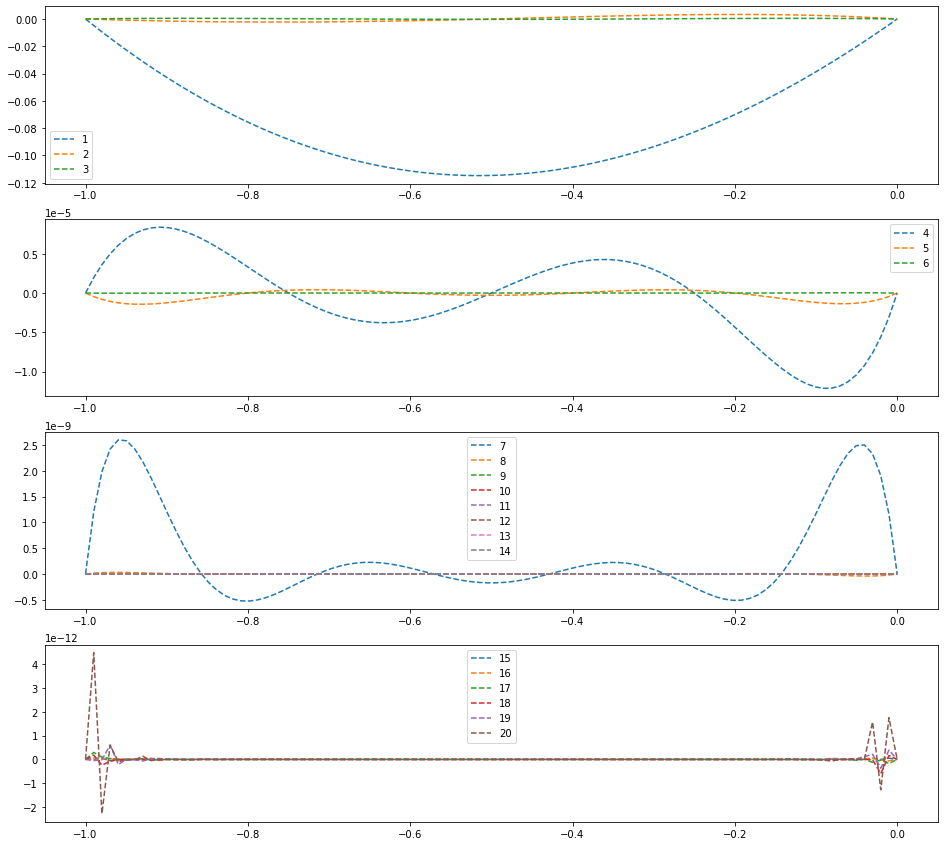
\includegraphics[width=\textwidth]{images/lagrange_equilateral_nodes}
\end{figure}

\newpage

Ստորև ներկայացված է $\delta_{n} \left(x\right) = f\left(x\right) - L_{n-1}\left(x\right)$ ֆունկցիաների գրաֆիկները օպտիմալ հանգույցների դեպքում։

\begin{figure}[h]
   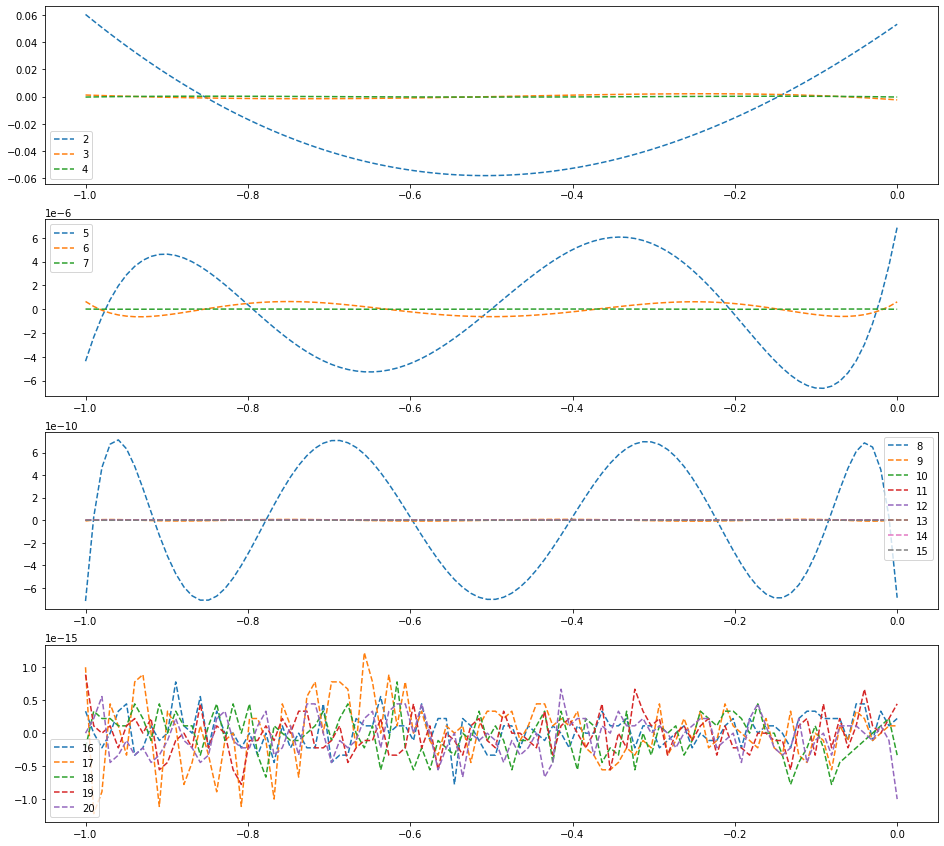
\includegraphics[width=\textwidth]{images/lagrange_optimal_nodes}
\end{figure}

\footnotetext{Բազմանդամերի հաշվումը և գրաֆիկերի կազմումը կատարվել է $Python$ ծրագրավորման լեզվի $NumPy$ և $MatPlotLib$ գրադարանների միջոցով։}


\newpage

\section*{Խնդիր 5}

Կառուցել քառակուսացման բանաձև $I$ անիսկական ինտեգրալը $\epsilon = 0.001$ ճշտությամբ հաշվելու համար։

						$$I = \int_{1}^{+\infty}\dfrac{\sin\left(x - 3\right)}{\sqrt[3]{x^{4}\left(2x+7\right)}}dx$$


\subsection*{Լուծում․}

Քառակուսացման բանաձև կառուցելու համար ինտեգրալը բաժանենք երկու մասի։


\begin{equation} \label{eq}
				I = \int_{1}^{\omega}\dfrac{\sin\left(x - 3\right)}{\sqrt[3]{x^{4}\left(2x+7\right)}}dx + \int_{\omega}^{+\infty}\dfrac{\sin\left(x - 3\right)}{\sqrt[3]{x^{4}\left(2x+7\right)}}dx
\end{equation}


$\omega$ ֊ն ընտրենք այնպես, որ (1) ֊ի ձախ ինտեգրալում սխալը չգերազանցի $\dfrac{\epsilon}{2}$ ֊ը։

		$$\int_{\omega}^{+\infty}\dfrac{\sin\left(x - 3\right)}{\sqrt[3]{x^{4}\left(2x+7\right)}}dx  \leq \int_{\omega}^{+\infty}\dfrac{1}{\sqrt[3]{x^{4}\left(2x+7\right)}}dx \leq
		\int_{\omega}^{+\infty} x ^ {-\sfrac{5}{3}} dx < \dfrac{\epsilon}{2} \implies -\frac{3}{2} x ^ {-\frac{2}{3}} \Big |_{\omega}^{+\infty}  < \dfrac{\epsilon}{2} \implies$$

		$$ \implies\frac{3}{2}\omega^{-\frac{2}{3}} < \frac{\epsilon}{2} \implies \omega > \left(\dfrac{\epsilon}{3} \right)^{-\sfrac{3}{2}} \approx 164317$$


Այսպիսով, եթե անիսկական ինտեգրալի փոխարեն հաշվենք (1) բանաձևի աջ մասի առաջին ինտեգրալը, ապա սխալը չի գերազանցի $\dfrac{\epsilon}{2}$֊ը։

Ինտեգրալը հաշվենք սեղանների բանաձևով, հավասարաչափ քայլերով։

							$$I = \int_{1}^{\omega}\dfrac{\sin\left(x - 3\right)}{\sqrt[3]{x^{4}\left(2x+7\right)}}dx \approx  \sum_{k = 0}^{N - 1} \dfrac{f\left(x_{k+1}\right) + f\left(x_{k}\right)}{2}\left(x_{k + 1} - x_{k}\right) \equiv \tilde{I}$$

							$$R_2 = M_{2} \dfrac{\left(b - a\right)h^{2}}{12} \implies h = \sqrt{\dfrac{12 \dfrac{\epsilon}{2}}{M_{2}\left(b - a\right)}}$$
					
								$$M_{2} = \underset{x \in \left[1, \omega\right]}{max}\left|f^{\left(2\right)}\left(x\right)\right| = \left|f^{\left(2\right)}\left(1\right)\right| \approx 0.456$$

Հետևաբար․
					
							$$h \approx 0.056$$
							$$\tilde{I} \approx -0.264177$$

Ինտեգրալի արժեքը՝  $$ I \approx -0.265111$$


\end{document}























